% Physics Homework Template
% Useful for completing homework questions from the textbook.
\documentclass[11pt]{homework}
\usepackage{siunitx}
\usepackage{amsmath}
\usepackage{tikz}
\usepackage{pgfplots}
\pgfplotsset{compat=1.18}

\newcommand{\hwname}{Corbin Hibler}
\newcommand{\hwemail}{c-hibler@onu.edu}
\newcommand{\hwtype}{Ch. 7 HW}
\newcommand{\hwnum}{}
\newcommand{\hwclass}{PHYS 2311}
\newcommand{\hwlecture}{0}
\newcommand{\hwsection}{Z}

\begin{document}
\maketitle

% MisConceptual Questions
\renewcommand{\questiontype}{MisConcQ}
\setcounter{questionCounter}{0}

\question
1. d\\
3. e\\
5. d\\
7. c\\
9. b\\
11. b\\
13. d

% Problems
\renewcommand{\questiontype}{Problem}
\setcounter{questionCounter}{0}

% Problem 1
\question
\[    
W= \vec{F_g}\cdot\Delta \vec{x}
\]\[
F_g = mg 
\]\[
W = mg \Delta x  = (280)(9.8)(3.80) = \boxed{\qty{10400}{J}}
\]

% Problem 2
\question
\[
W = \vec{F}\cdot \Delta\vec{x}
\] \[
\Delta x = \frac{W}{F_g} = \frac{W}{mg} = \frac{70.0}{(1.85)(9.8)} = \boxed{\qty{3.86}{m}}
\]

% Problem 5
\setcounter{questionCounter}{4}
\question
\[
m = \qty{46.0}{kg}, \quad \Delta x = \qty{10.3}{m}, \quad \mu_k = 0.40
\]\[
W = \vec{F}\cdot \Delta\vec{x}
\]\[
\vec{F}=F_{app} - f_k = 0
\]\[
f_k = F_N\mu_k = mg\mu_k = (46.0)(9.8)(0.40) = \qty{180.32}{N}
\] \[
\implies F_{app} = \qty{180.32}{N}
\]\[
W = (180.32)(10.3) = \boxed{\qty{1860}{J}}
\]
% Problem 8
\setcounter{questionCounter}{7}
\question
\[
    m = \qty{950}{kg}, \quad \Delta x = \qty{510}{m}, \quad \theta = \qty{9.0}{\degree}
\]\[
F_g=mg \sin \theta
\]\[
W = mg \sin \theta \Delta x
\]
\[
    W = (950)(9.8)\sin(9.0)(510) = \boxed{\qty{7.4e5}{J}}
\]
% Problem 12
\setcounter{questionCounter}{11}
\question
\[
\vec x(t)=\vec x_0+\vec v_0t+\frac{1}{2}\vec at^2
\]\[
    \Delta x = \frac{1}{2}at^2 
\]\[
F = ma
\]
\[
    W = F\Delta x = \frac{1}{2}a^2t^2m = \frac{1}{2}(2.0)^2(8.0)^2(4.0) = \boxed{\qty{512}{J}}
\]

% Problem 18
\setcounter{questionCounter}{17}
\question
\[
    \vec{A} \cdot \vec{B} = (2.0x^2)(11.0) + (-4.0x)(2.5x) + (5.0)(0) 
\]
\[
    = 22x^2 - 10x^2 = \boxed{12x^2 \text{ units}}
\]

% Problem 20
\setcounter{questionCounter}{19}
\question
\[
    \vec{A} \cdot \vec{B} = (5.8)(8.2) + (-3.4)(4.3) + (-6.2)(-7.0) = 76.34
\]\[
|\vec{A}| = \sqrt{(5.8)^2+(-3.4)^2+(-6.2)^2} = 9.15
\]\[
|\vec{B}| = \sqrt{(8.2)^2+(4.3)^2+(-7.0)^2} = 11.61
\]\[
\theta = \arccos\left(\frac{A \cdot B}{|A||B|}\right) 
\]
\[
    \theta = \arccos\left(\frac{76.34}{9.15 \cdot 11.61}\right) = \boxed{\qty{44.2}{\degree}} 
\]

% Problem 22
\setcounter{questionCounter}{21}
\question
\[
    \vec{V_1} = 0 \hat{i} + 75 \hat{k}
\]
\[
    \vec{V_2} = 48\cos(-48) \hat{i} + 48\sin(-48) \hat{k} = 32.11 \hat{i} - 35.67 \hat{k}
\]
\[
    \vec{V_1} \cdot \vec{V_2} =  (0)(32.11) + (75)(-35.67) = \boxed{\qty{-2675}{units}}
\]

% Problem 25
\setcounter{questionCounter}{24}
\question
\begin{alphaparts}
\questionpart
\[
    \vec{B} + \vec{C} = (-8.0 + 5.8)\hat{i} + (6.1-9.2)\hat{j} + 4.2 \hat{k} = -2.2 \hat{i} -3.1 \hat{j} +4.2 \hat{k}
\]
\[
    \vec{A} \cdot (\vec{B}+\vec{C}) = (9.0)(-2.2) + (-8.5)(-3.1) + (0)(4.2) = \boxed{6.55}
\]
\questionpart
\[
    \vec{A}+\vec{C} = (9.0+5.8)\hat{i} + (-8.5-9.2)\hat{j} = 14.8\hat{i} - 17.7 \hat{j}   
\]\[
\vec{B} \cdot (\vec{A}+\vec{C}) = (-8.0)(14.8) + (6.1)(-17.7) + (4.2)(0) = \boxed{-226}
\]
\questionpart
\[
    \vec{B}+\vec{A} = (-8.0+9.0)\hat{i} + (6.1-8.5)\hat{j} + (4.2+0)\hat{k} = 1\hat{i} - 2.4 \hat{j} + 0\hat{k}
\]
\[
    (\vec{B}+\vec{A}) \cdot \vec{C} = (1)(5.8) + (-2.4)(-9.2) + (0)(0) = \boxed{27.9}
\]


\end{alphaparts}

% Problem 37
\setcounter{questionCounter}{36}
\question

\centering
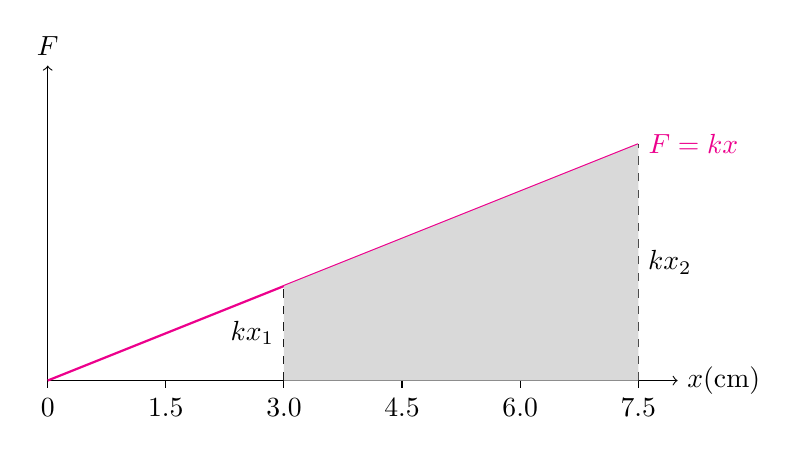
\begin{tikzpicture}
    % Axes
    \draw[->] (0,0) -- (8,0) node[right] {$x$(cm)};
    \draw[->] (0,0) -- (0,4) node[above] {$F$};
    
    % Force line F = kx
    \draw[thick, magenta] (0,0) -- (7.5,3) node[right] {$F = kx$};
    
    % Dashed lines showing heights at x = 3.0 and x = 7.5
    \draw[dashed] (3.0,0) -- (3.0,1.2);
    \draw[dashed] (7.5,0) -- (7.5,3);
    
    % Labeling the height at x = 3.0 and x = 7.5 as kx
    \node[right] at (7.5,1.5) {$kx_2$};
    \node[left] at (3.0,0.6) {$kx_1$};
    
    % Adjusted shaded region under the curve between x = 3.0 and x = 7.5
    \fill[gray!30] (3.0,0) -- (3.0,1.2) -- (7.5,3) -- (7.5,0) -- cycle;
    
    % Labeling x-axis length
    \foreach \x in {0, 1.5, 3.0, 4.5, 6.0, 7.5} {
        \draw (\x, 0) -- (\x, -0.1) node[below] {\x};
    }
    
\end{tikzpicture}
\[
    W = \int_{0.03}^{0.075}65x = \frac{1}{2}65x^2\Big|_{0.03}^{0.075} = \frac{1}{2}(65)(0.075)^2 - \frac{1}{2}(65)(0.03)^2 = \boxed{\qty{0.15}{J}} 
\]

% Problem 39
\setcounter{questionCounter}{38}
\question



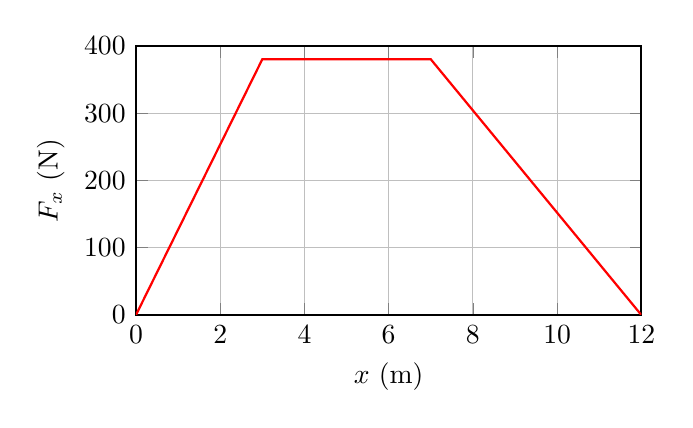
\begin{tikzpicture}
    \begin{axis}[
        width=8cm, height=5cm,
        grid=major,
        xlabel={$x$ (m)},
        ylabel={$F_x$ (N)},
        xmin=0, xmax=12,
        ymin=0, ymax=400,
        xtick={0,2,4,6,8,10,12},
        ytick={0,100,200,300,400},
        thick,
    ]
        % Plot the force vs distance graph
        \addplot[red, thick] coordinates {
            (0, 0) 
            (3, 380) 
            (7, 380) 
            (12, 0) 
        };
    \end{axis}
\end{tikzpicture}
\[
    W = \frac{1}{2}(380)(3) + (380)(4) + \frac{1}{2}(380)(5) = \boxed{\qty{3040}{J}}
\]

% Problem 41
\setcounter{questionCounter}{40}
\question
\begin{alphaparts}
\questionpart
\[
    W = \frac{1}{2}(400)(3) + (400)(4) + \frac{1}{2}(400)(3) = \boxed{\qty{2800}{J}}
\]
\questionpart
\[
    W = \frac{1}{2}(-200)(1.5) + (-200)(2) + \frac{1}{2}(-200)(1.5) = \qty{-700}{J}
\]
\[
    \qty{2800}{J} - \qty{700}{J} = \boxed{\qty{2100}{J}}
\]
\end{alphaparts}

% Problem 45
\setcounter{questionCounter}{44}
\question
\[
    W = \int_{0.0}^{1.0}\frac{3.0}{\sqrt{x}}=3.0 \int_{0.0}^{1.0}x^{-\frac{1}{2}}=3.0 \cdot 2x^{\frac{1}{2}}\Big|_{0.0}^{1.0} = 3.0 \cdot (2(1)^{\frac{1}{2}}) = 3.0 \cdot 2 = \boxed{\qty{6.0}{J}}
\]

% Problem 55
\setcounter{questionCounter}{54}
\question
\begin{alphaparts}
\questionpart
\[
    3K_i = K_f
\]
\[
    3(\frac{1}{2}mv_i^2) = \frac{1}{2}mv_f^{2}  
\]
\[
    3v_i^2 = v_f^2 
\]
\[
    \sqrt{3}v_i = v_f
\]
\[
    \implies \boxed{\sqrt{3}}
\]
\questionpart
\[
    K=\frac{1}{2}m\left(\frac{v}{2}\right)^2 = \frac{1}{8}mv^2=\frac{1}{4}\left(\frac{1}{2}mv^2\right) = \frac{K}{4}
\]\[
\implies \boxed{\frac{1}{4}}
\]
\end{alphaparts}

% Problem 56
\question
\[
W_{\text{net}}= W_{\text{stop}} - W_{\text{moving}} = 0
\]\[
W_{\text{stop}} = W_{\text{moving}}
\]\[
W_{\text{net}} = \Delta K
\]
\[
K_{\text{stop}} = W_{\text{stop}}
\]\[
K_{\text{stop}} = \frac{1}{2}mv^2 = \frac{1}{2}(\qty{9.11e-31})(\qty{1.10e6})^2 = \boxed{\qty{5.51e-19}{J}}
\]

% Problem 59
\setcounter{questionCounter}{58}
\question
\[
    W = F \Delta x
\]
\[
    F = \frac{W}{\Delta x}
\]
\[
    W = K = \frac{1}{2}mv^2 
\]
\[
    F = \frac{\frac{1}{2}mv^2}{\Delta x} = \frac{\frac{1}{2}(0.145)(32)^2}{0.22} = \boxed{\qty{337.5}{N}}
\]

% Problem 60
\question
\[
    m = \qty{0.085}{kg}, \quad F = \qty{105}{N}, \quad \Delta x = \qty{0.75}{m}
\]\[
    W = F \Delta x = K = \frac{1}{2}mv^2
\]\[
F \Delta x = \frac{1}{2}mv^2 
\]\[
\sqrt{\frac{2F\Delta x}{m}} = v 
\]\[
v = \sqrt{\frac{2(105)(0.75)}{0.085}} = \boxed{\qty{43.0}{m/s}}
\]

% Problem 65
\setcounter{questionCounter}{64}
\question
\[
    \Delta x = \qty{8.0}{m}, \quad v_i = \qty{5.0}{m/s}, \quad v_f = \qty{0}{m/s}
\]\[
f_k = F_N\mu_k
\]\[
W = f_k \Delta x
\]\[
W=\Delta K=\frac{1}{2}mv_{f}^2-\frac{1}{2}mv^2_{i} = \frac{1}{2}m(v_f^2 - v_i^2)
\]\[
\frac{1}{2}m(v_f^2-v_i^2) = F_N\mu_k \Delta x
\]\[
F_N = mg
\]\[
\frac{\frac{1}{2}m(v_f^2-v_i^2)}{mg\Delta x} = \mu_k
\]\[
\mu_k = \frac{v_f^2-v_i^2}{2g\Delta x} = \frac{0+25.0}{2(9.8)(8.0)} = \boxed{0.16}
\]




\end{document}
